\documentclass[../main.tex]{subfiles}
\graphicspath{
    {"../img/"}
    {"img/"}
}

\begin{document}
\subsection{Dystrybucje}
    \begin{definicja}
        Niech $D$ - przestrzeń funkcji klasy $\mathcal{C}^\infty(\mathbb{R})$ o zwartym nośniku. Czyli
        \[
            \underset{K\subset\mathbb{R}}{\exists} ,\text{$K$ - domknięty},\quad \underset{\varphi\in D}{\forall} \quad \underset{x\not\in K}{\forall} \varphi(x) = 0
        .\]
    Przestrzeń $D$ nazywamy przestrzenią funkcji próbnych.
    \end{definicja}
    \begin{przyklad}
        $\varphi\in D$
        \[
            \varphi(x) = \begin{cases}
                e^{-\frac{1}{1-x^2}}&-1\le x \le 1\\
                0 & x\not\in[-1,1]
            \end{cases}
        .\]
    \end{przyklad}
    Przestrzeń dualną do $D$ oznaczymy przez $D^\star$
     \begin{definicja}
        Funkcjonał liniowy z przestrzeni $D^\star$ nazywamy dystrybucją.
        \textbf{Oznaczenia:} jeżeli $T\in D^\star$, $\varphi\in D$, to
         \[
             T(\varphi) \overset{\text{ozn}}{=} \left<T, \varphi \right>
         .\]
    \end{definicja}
    \begin{przyklad}
        Niech
        \[
            \theta(x) = \begin{cases}
                1 & x \ge 0\\
                0 & x < 0
            \end{cases}
        .\]
    $T_\theta$ jest dystrybucją. Wówczas
        \[
            \left<T_\theta, \varphi \right> \overset{\text{def}}{=} \int\limits_{-\infty}^{\infty} \theta(x)\varphi(x)dx = \int\limits_{0}^{\infty} \varphi(x)dx
        .\]
    \end{przyklad}
    Oznacza to, że jeżeli $f$ - funkcja na $\mathbb{R}$, to możemy z nią związać dystrybucję $T_f\in D^\star$ taką, że
    \[
        \left<T_f, \varphi \right> = \int\limits_{-\infty}^{\infty} f(x)\varphi(x)dx
    .\]

\pagebreak
\begin{definicja}
    Niech $T\in D^\star$, wówczas przez $T'$ oznaczymy dystrybucję o następującej własności
    \[
        \underset{\varphi\in D}{\forall} \left<T', \varphi \right> = -\left<T, \varphi' \right>
    .\]
\end{definicja}
\textbf{Uwaga: } powyższa definicja spełnia warunek
\[
    \left( T_f \right)' = T_{f'}
,\]
bo
\[
    \int\limits_{-\infty}^{\infty} f'(x)\varphi(x)dx = f(x)\varphi(x)\Big|_{-\infty}^{+\infty} - \int\limits_{-\infty}^{\infty} f(x)\varphi'(x) dx = -\int\limits_{-\infty}^{\infty} f(x)\varphi'(x)dx
.\]
Dalej
\[
    \left<T'_f, \varphi \right> = -\left<T_{f}, \varphi' \right> = -\int\limits_{-\infty}^{\infty} f(x)\varphi'(x)dx
.\]
\begin{definicja}
    Niech $\delta \in D^\star$. Dystrybucję $\delta$ nazywamy deltą Diraca i definiujemy tak:
    \[
        \left<\delta, \varphi \right> \overset{\text{def}}{=} \varphi(0)
    .\]
Analogicznie,
\[
    \left<\delta_a, \varphi \right>\overset{\text{def}}{=} \varphi(a)
.\]
\end{definicja}
\begin{definicja}
Czasami pojawiają się takie oznaczenia (konwencje):
\begin{align*}
    \delta &= \delta(x)\\
    \delta_a &= \delta(x-a)\\
    \left<\delta, \varphi \right> &= \int\limits_{-\infty}^{\infty} \delta(x)\varphi(x)dx\\
    \left<\delta_a, \varphi \right> &= \int\limits_{-\infty}^{\infty} \delta(x-a)\varphi(x)dx
.\end{align*}
Można też znaleźć takie napisy:
\[
    \delta(x) = \begin{cases}
        \infty & x = 0\\
        0 & x \neq 0
    \end{cases}
.\]
\[
    \int\limits_{-\infty}^{\infty} \delta(x)dx = 1
.\]
\textbf{Obserwacja:}
\[
    \int\limits_{-\infty}^{\infty} 7\delta(x)dx = 1 \neq 7 \int\limits_{-\infty}^{\infty} \delta(x)dx = 7
,\]
a ona miała być elementem przestrzeni liniowej.
\end{definicja}
Policzmy $\left( T_\theta \right)'$.
\[
    \left<T'_{\theta}, \varphi \right> =- \left<T_\theta, \varphi' \right>
.\]
Prawa strona:
\begin{align*}
    -\left<T_\theta, \varphi' \right> &= -\int\limits_{-\infty}^{\infty} \theta(x)\varphi'(x)dx = -\int\limits_{-\infty}^{\infty} \varphi'(x)dx = -\varphi(x)\Big|_{0}^{\infty} =\\
    &= - \lim_{x \to \infty}\varphi(x) + \varphi(0) = \varphi(0) = \left<\delta, \varphi \right>
.\end{align*}
\[
    \left( T_\theta \right)' = \delta
.\]
\[
    "\theta' = \delta"
.\]
Ale to nie ma sensu, ale na poziomie
\[
\underset{\varphi\in D}{\forall}     \left<T_{\theta'},\varphi \right> = \left<\delta, \varphi \right>
\]
też nie, ale trochę mniej.
\[
    \left<\left( T_{\theta} \right)', \varphi \right> = \left<\delta, \varphi \right>
\]
sens ma, ale w literaturze pojawiają się wszystkie 3 napisy.
\begin{przyklad}
Niech $E$ - pole elektryczne.
\begin{figure}[h]
    \centering
    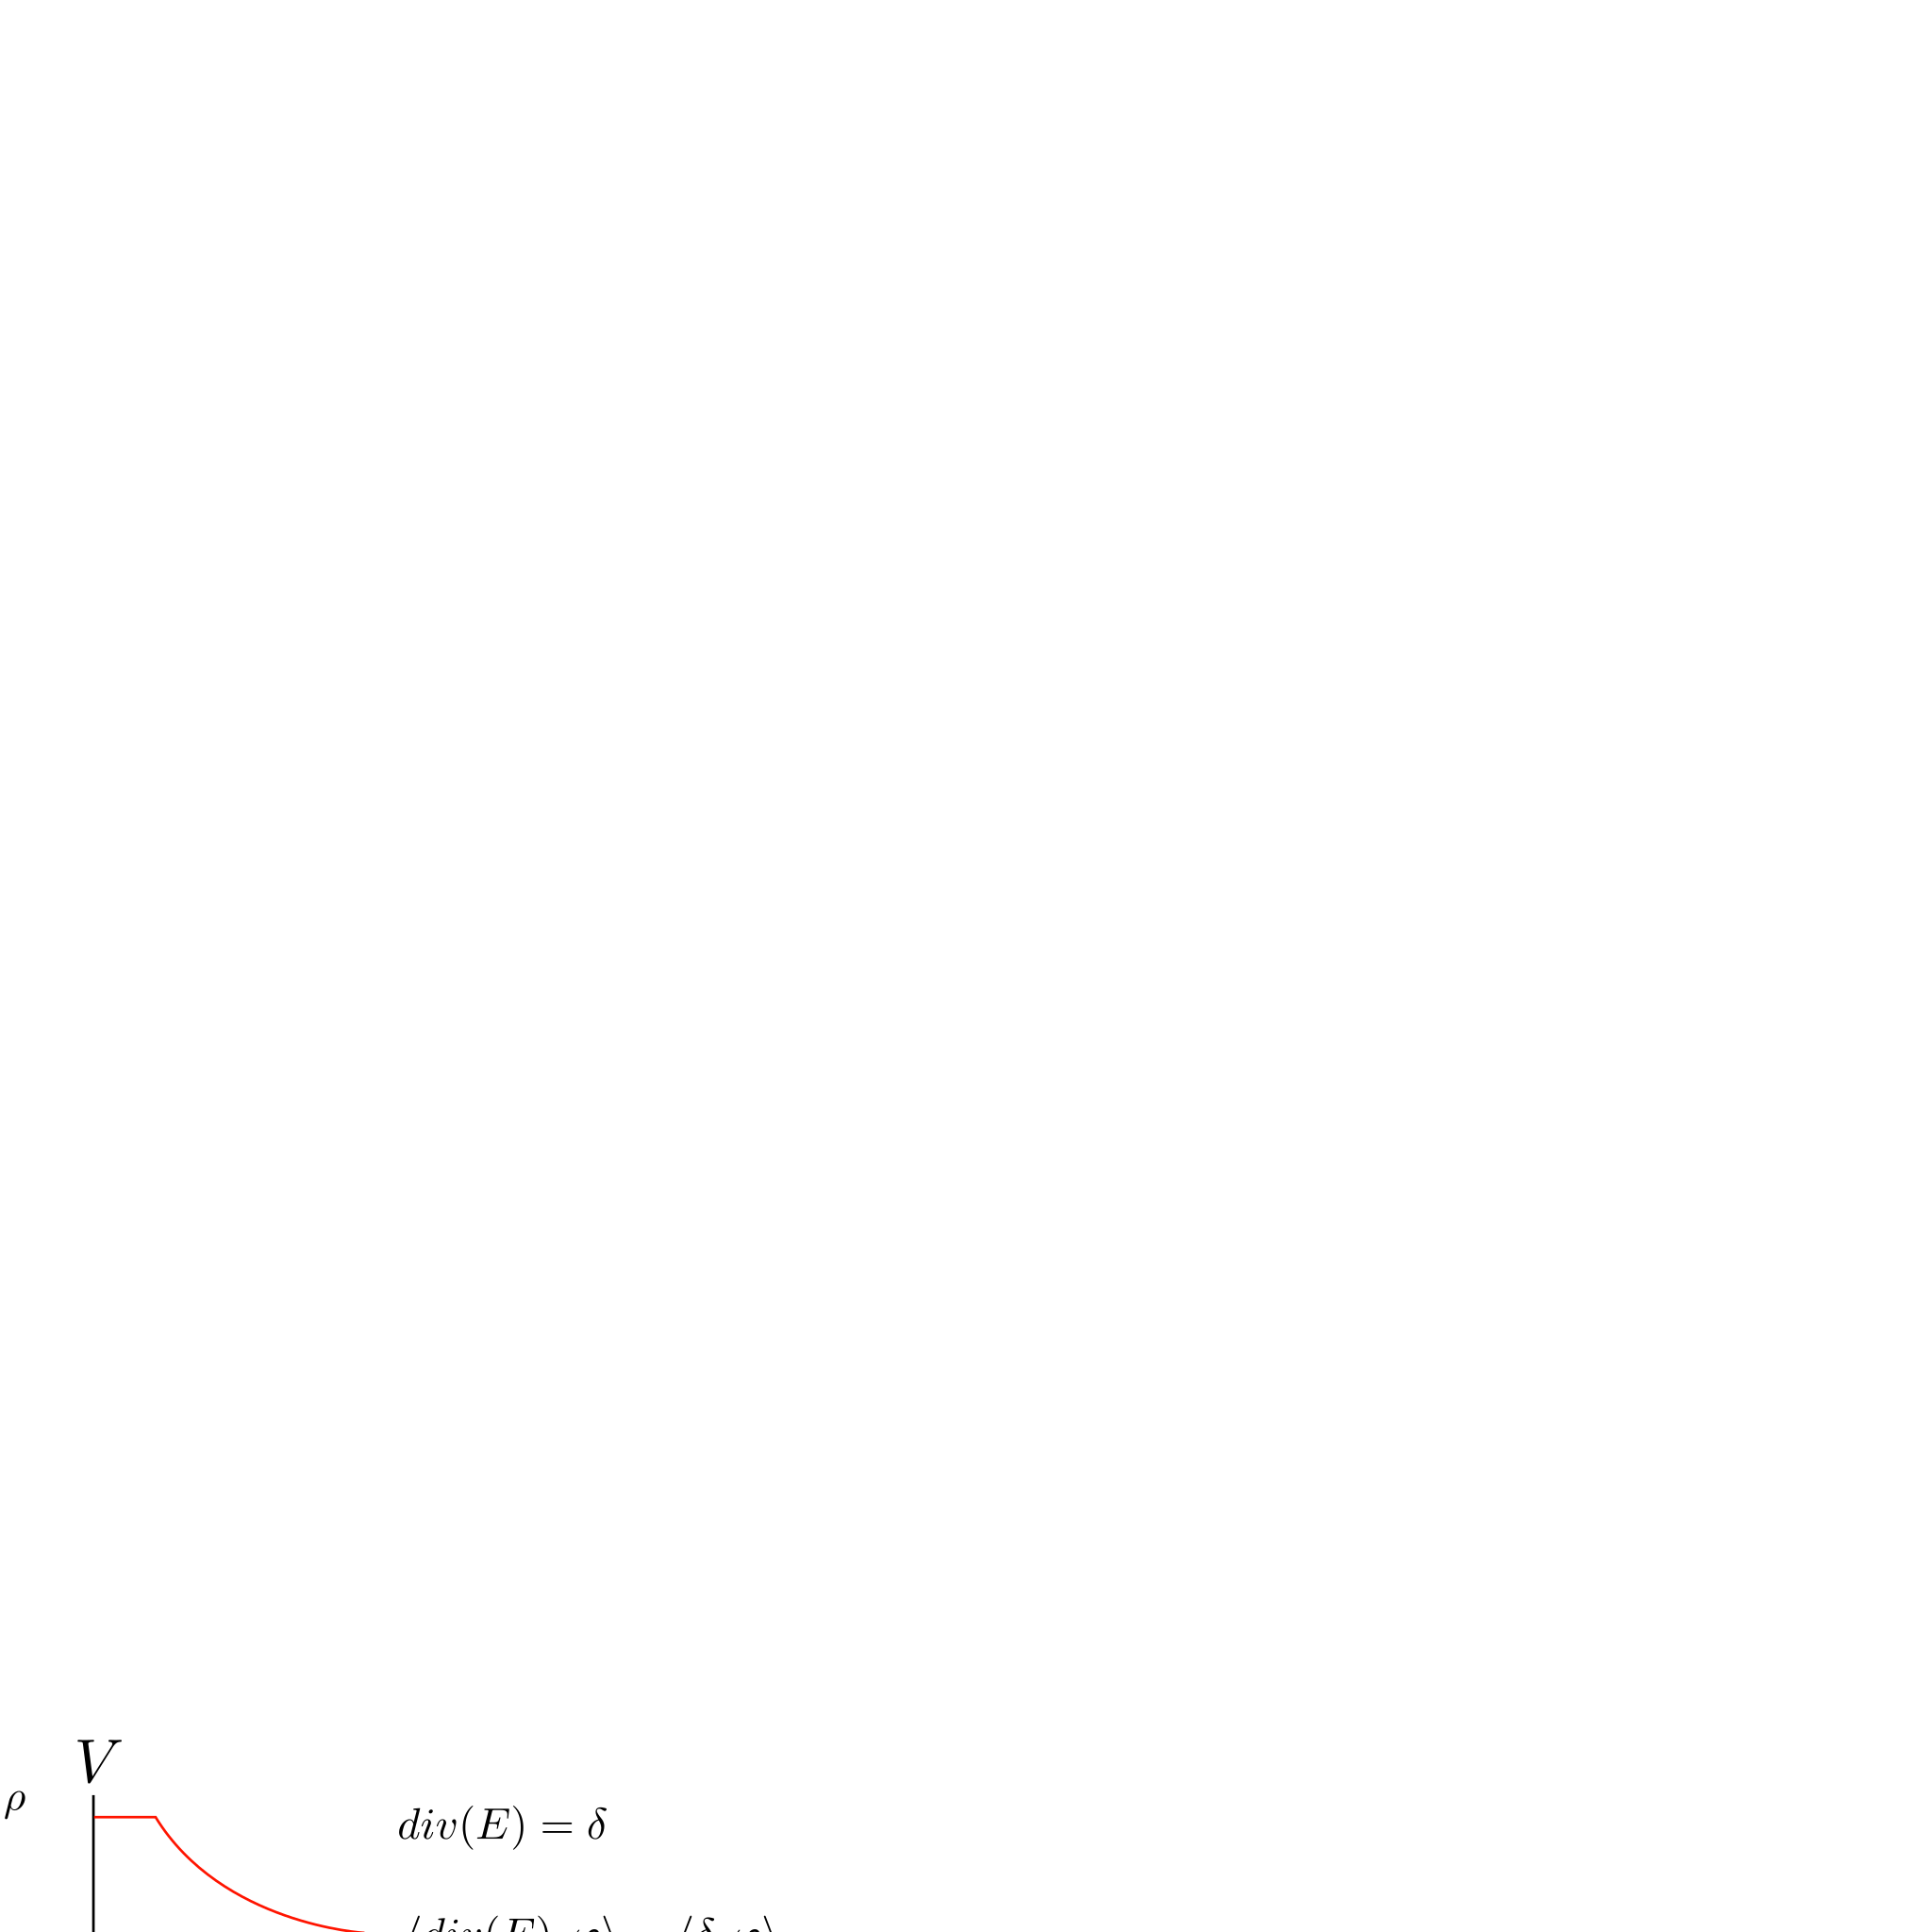
\includegraphics[width=\textwidth]{w24-1}
    \caption{Dlaczego fizycy lubią deltę Diraca?}
    \label{fig:w24-1}
\end{figure}
\[
    \left<T_f, \varphi \right> = \int\limits_{-\infty}^{\infty} f(x)\varphi(x)dx
.\]
\end{przyklad}
\begin{definicja}
    Niech $f: \mathbb{R}\to \mathbb{R}$, taka, że dla $x = a$
    \[
        \lim_{x \to a^+} f(x) - \lim_{x \to a^-}f(x) = \sigma
    .\]
(Kiedyś poważniejszą wersję tego nazywaliśmy wahaniem funkcji)
\end{definicja}
Policzmy $\left( T_f \right)'$
\begin{align*}
    \left<\left( T_f \right)', \varphi \right> &= -\left<T_f, \varphi' \right> = -\int\limits_{-\infty}^{\infty} f(x)\varphi'(x)dx =\\
    &=-\int\limits_{a}^{\infty} f(x)\varphi'(x)dx - \int\limits_{-\infty}^{a} f(x)\varphi'(x)dx =\\
    &= -f(x)\varphi(x)\Big|_{a}^\infty  + \int\limits_{a}^{\infty} f'(x)\varphi(x)dx +\\
    &- f(x)\varphi(x)\Big|_{-\infty}^a + \int\limits_{-\infty}^{a} f'(x)\varphi(x)dx  =\\
    &= \lim_{x \to a^+}f(x)\varphi(x) - \lim_{x \to a^-}f(x)\varphi(x) +\\
    &+ \underset{\text{bez $x = a'$ }}{\int\limits_{-\infty}^{\infty} f'(x)\varphi(x)dx} = \underbrace{\sigma \varphi(a) + \int\limits_{-\infty}^{\infty} \left\{ f'(x) \right\} \varphi(x)dx}_{\clubsuit} = \\
    &= \left<\sigma \cdot \delta + T_{\left\{ f' \right\} }, \varphi \right>
.\end{align*}
Czyli niepoprawnie piszemy tak:
\[
    f' = \sigma \cdot \delta + \left\{ f' \right\}
\]
i rozumiemy w sensie $\clubsuit$
\begin{przyklad}
    Rozwiązać równanie
    \[
        f''(x) + \omega^2 f(x) = \delta(x-a)
    .\]
Bierzemy dwie funkcje:
\begin{align*}
    f_1(x) &= A_1 \sin(\omega x) + B_1\cos(\omega x) & x < a\\
    f_2(x) &= A_2 \sin(\omega x) + B_2\cos(\omega x) & x > a\\
    f_1(a) &= f_2(a)\\
    \lim_{x \to a} f_2'(x)& - f_1'(x) = 1
.\end{align*}
Zatem
\begin{align*}
    A_1 \sin(\omega a) + B_1 \cos(\omega a) &= A_2 \sin(\omega a) + B_2 \cos(\omega a)\\
    \omega A_1 \cos(\omega a) - B_1 \omega \sin(\omega a) &= \omega A_2 \cos(\omega a) - B_2 \omega \sin (\omega a) - 1
.\end{align*}
    W szczególności ($B_1 = 0$, $A_2 = 0$)
    \begin{align*}
        A_1\sin(\omega a) &= B_2 \cos(\omega a)\\
        \omega A_1 \cos(\omega a) &= -B_2 \omega \sin(\omega a) - 1
    .\end{align*}
    Więc
    \[
        f(x) = \begin{cases}
            --------- & x > a\\
            --------- & x < a
        \end{cases}
    .\]
\end{przyklad}
\subsection{Zastosowania}
Mamy coś takiego
\begin{equation}
    \label{eqn:w24-1}
    x''(t) + \omega^2 x(t) = h(t) \tag{$\star$}.
\end{equation}
Wiemy, że $f''(t) + \omega f(t) = \delta(x-a)$. Niech
\[
    x(t) = \int\limits_{-\infty}^{\infty} f(s)h(t-s)ds =  \left<T_f, h_t \right>
.\]
Czym jest $\dot{x}(t)$?
\[
    \left<\dot{x}(t),\varphi \right> = \left<T_{f'}, \varphi \right>
,\]
\[
    \left<\ddot{x}(t), \varphi \right> = \left<T_{f''}, \varphi \right>
.\]
Wówczas
\begin{align*}
    \left<x'' + \omega x', h \right> &= \left<T_{f'} + \omega^2 T_f, h \right> = \int\limits_{-\infty}^{\infty} \left( (f'' + \omega^2 f)h \right) =\\
    &= \left<\delta(t,a), h \right> = h(t)
.\end{align*}



\end{document}
